\chapter{Immersive Environments: XR}
\label{ch:xr-mus}

%Finally, \textbf{Chapter \ref{ch:xr-mus}} discusses how contemporary extended reality (XR) systems can be exploited to enhance the musical experience of multi-channel music. Our main focus here is to present how XR can be used as a dissemination tool allowing the public greater access to this type of music. As a way to contrast the access issue surrounding XR, and in order to be thorough, we will also discuss some XR tools that are not as low-cost or open-source.

In chapter \ref{ch:spat-mus} we discussed tools for the creation of spatial music from a computer-music standpoint, with a focus on FOSS. Furthermore, we explored spatial instruments which facilitate the creation of such music works. Later, in chapter \ref{ch:spat-aud}, we focused on recording and reproduction means for spatial audio. In particular, we focused on ambisonic recording and reproduction tools, given their popularity in the open-source community interested in spatial audio. In this chapter, we would like to discuss how Extended Reality (XR) tools can also be used as for reproduction of spatial audio works. 

A large motivation for the creation and dissemination of spatial music stems from the growth of the XR industry in the last decade. Any complete discussion involving spatial music therefore, should address how spatial music is being shaped by the development of these new tools. Over the years a number of scientists and companies have developed increasingly sophisticated XR systems in academic and commercial settings. Unfortunately, many of the more sophisticated XR system still remain too costly for most people in the world.

Our intention is to shed a light on all the different types of XR technologies while focusing particular attention on technologies that allow for low-cost and open-source dissemination of spatial audio. We believe the WebXR is a powerful distribution tool which could be adopted by many artists working in the spatial audio domain. Online publishing is an important part of any artists work, allowing people to preview their work before committing to a live experience. WebXR provides musicians working with spatial music the opportunity to reach a wide audience, while preserving some of the depth that was carefully crafted into their music.

\section{The History of VR}

LaValle defines VR in the introductory chapter of his book "Virtual Reality" \cite{lavalle2016virtual}: 

\begin{enumerate}
    \item \textbf{Targeted behavior:} The organism is having an “experience” that was designed by the creator. Examples include flying, walking, exploring, watching a movie, and socializing with other organisms.
    \item \textbf{Organism:} This could be you, someone else, or even another life form such as a fruit fly, cockroach, fish, rodent, or monkey (scientists have used VR technology on all of these!).
    \item \textbf{Artificial sensory stimulation:} Through the power of engineering, one or more senses of the organism become co-opted, at least partly, and their ordinary inputs are replaced or enhanced by artificial stimulation.
    \item \textbf{Awareness}: While having the experience, the organism seems unaware of the interference, thereby being “fooled” into feeling present in a virtual world. This unawareness leads to a sense of presence in an altered or alternative world. It is accepted as being natural.
\end{enumerate}

In essence, every XR experience is simply a \textit{perceptual illusion}. A programmer creates an environment that attempts to fool another person's senses. It should be noted however, that this does not always mean the end goal is to make XR experiences as realistic as possible. Animations and graphic scenes are not only popular, but sometimes preferable to extremely realistic simulations.

In contrast to Mixed Reality (MR) and Augmented Reality (AR), VR experiences completely block out real-world sensory stimuli. Unfortunately, the definitions for AR and MR are quite loose today. It is more common for both consumers and companies to lump together AR and MR into a single category. It would appear that the typical consumer has become more familiar with the term AR, and a result it makes more financial sense to commercialize a MR system using this alternate label.

In general, AR and MR today have become synonymous. Some prefer to call simple \textit{overlay} applications AR, while reserving MR for more sophisticated systems which require \textit{machine vision}. For example, in a MR experience, an avatar that is displayed in your Field of View (FoV) might fall off a real table, and respond to this event. In an AR experience, in contrast, we might see a simple display of time, temperature, and humidity on one's viewer. This information then gets automatically updated as the user moves from one location to the next. In these AR systems there is no link between the geometrical space, and the objects inside it, and the system. 

Schmalstieg and Hollerer\cite{schmalstieg2016augmented} authored a comprehensive review of AR in their book: "Augmented reality: principles and practice". According to the authors AR implies the confluence of three elements:

\begin{enumerate}
    \item Combination of real and virtual worlds. 
    \item Interaction in real-time.
    \item Registration in 3D space. 
\end{enumerate}

The first part and second part of this definition are quite clear: the system must bring together elements of the real and synthetically generated world, and the system must respond to user interaction. The last element refers to the link between the physical and virtual world. In our previous example, the data from the real world is limited to time, temperature, and humidity. However, in more sophisticated MR experiences machine vision often provides a map of the space, which can then interact with the digital world. 

Milgram and Kishino described in 1994 a continuum which can help categorize different XR experiences \cite{schmalstieg2016augmented}. Figure \ref{fig:continuum} shows this spectrum. The term AR here, refers to systems that are more real than virtual. \textit{Augmented virtuality}, refers to systems that are more virtual than real. For example, we can imagine computer generated worlds where avatars faces are real, but the rest of the environment is digital.

\begin{figure}[ht!]%force figure here, top, strict
\centering
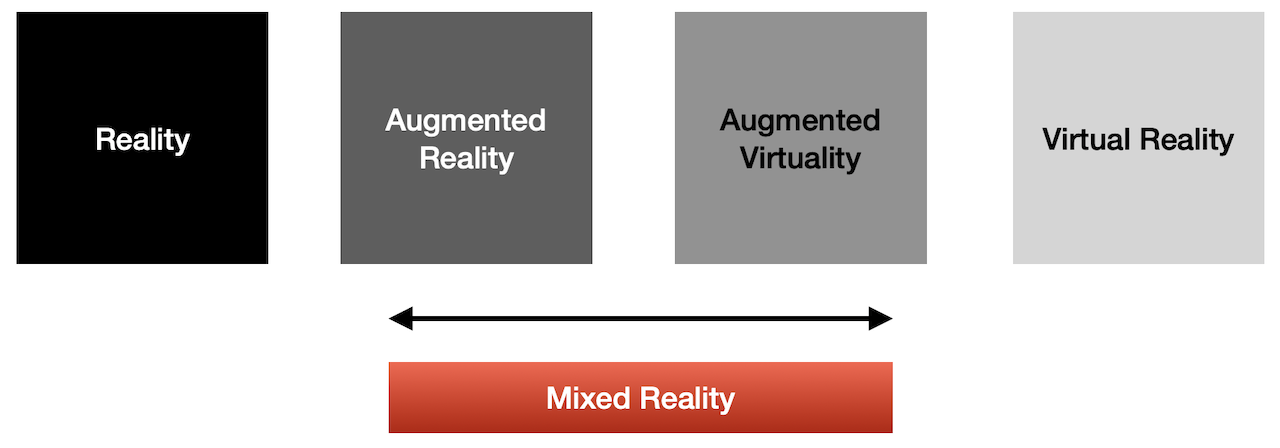
\includegraphics[width=0.7\textwidth]{img/continuum.png} 
%\captionsetup{justification=centering}
\caption{Milgram and Kishino Continuum}
\label{fig:continuum}
\end{figure}

In this definition, MR is anything that combines the real and virtual world. In general in this text, we will use AR and MR interchangeably. However, it should be noted, that there are still discrepancies in the use of the words. This phenomenon can be explained by the fact that these technologies are still quite young. In addition, new technologies are continually being developed, making categorization even harder.

Much before the first ever "real" VR experience was ever developed, pioneering painters, from as early as the 15th century, were already working on the concept of depth perception and optical perspective. Today we take for granted the idea that 2D representations of 3D space contain any dimensionality, but before the establishment of cameras, this was a feature which had to be creatively articulated by artists. The idea of a \textit{vanishing point}, the point at which receding parallel lines viewed in perspective appear to converge, shaped an entire generation of painters. Figure \ref{fig:san-pedro} shows Pietro Perugino's use of perspective in the "Entrega de las Llaves a San Pedro" fresco at the Sistine Chapel (1481–82).

In 1838, the first stereoscope was invented by Charles Wheatstone \cite{hemstrom2020comparison}. A stereoscope is a device in which a pair of images is presented to each eye in order to provide the illusion of depth. By the 1930s, a portable version of a stereoscope called the View-Master became commercially successful. One of the innovations of this device was the increased field of view (FoV) and blocking of distracting boundary stimulus to increase immersion. In 1957, Morton Heilig introduced the Sensorama which added motion pictures, stereo sound, vibration, wind, and even smells in a personalized stereoscopic multi-modal experience. Unfortunately, the Sensorama had a fixed perspective, which meant the user was limited to a single orientation. It was also very large and expensive, which ultimately led to its downfall.

\begin{figure}[ht!]%force figure here, top, strict
\centering
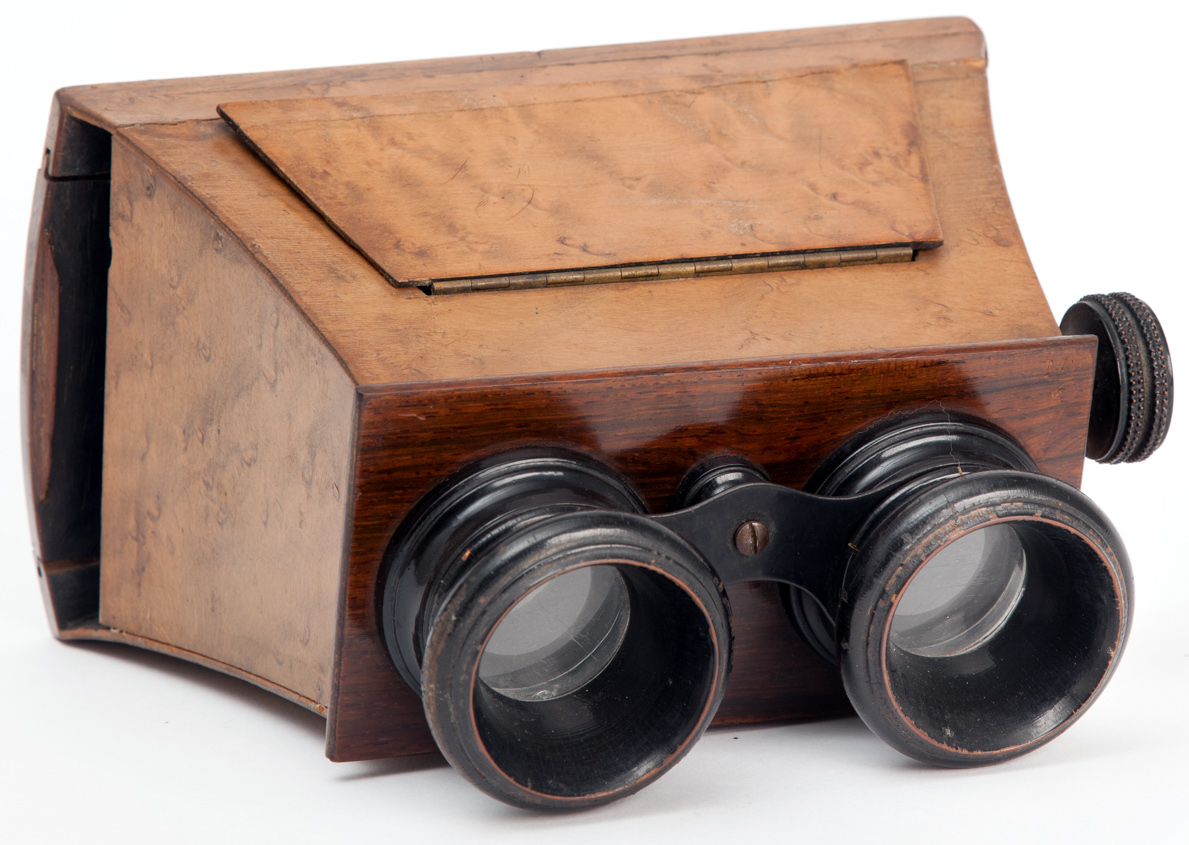
\includegraphics[width=0.7\textwidth]{img/stereoscope.jpg} 
%\captionsetup{justification=centering}
\caption{Brewster-type\protect\footnotemark stereoscope, 1870 \cite{FileIGB032online}}
\end{figure}

\footnotetext{Sir David Brewster (11 December 1781 – 10 February 1868) was a Scottish scientist, inventor, author, and academic administrator.}

Then, in 1878, one of the first examples of of \textit{stroboscopic apparent motion} was created by Eadward Muybridge\footnote{Muybridge was an English photographer important for his pioneering work in studies of photographic motion (9 April 1830 – 8 May 1904)}. This effect refers to the ability to generate apparent motion by flipping through a sequence of images at a fast rate. Figure \ref{fig:horse-motion} shows Muybridge's famous work "The Horse in Motion", depicting several "frames" of a horse as it seemingly moves across space. For this sequence 24 cameras were used, these were triggered by the horse as it moved along a track. In order to reproduce the images a \textit{zoopraxiscope}, also an invention of Muybridge, was used. The zoopraxiscope is a disc containing multiple image frames which is used to project a moving image in a recirculating fashion \cite{lavalle2016virtual}.

\begin{figure}[!htb]
\minipage{0.5\textwidth}
  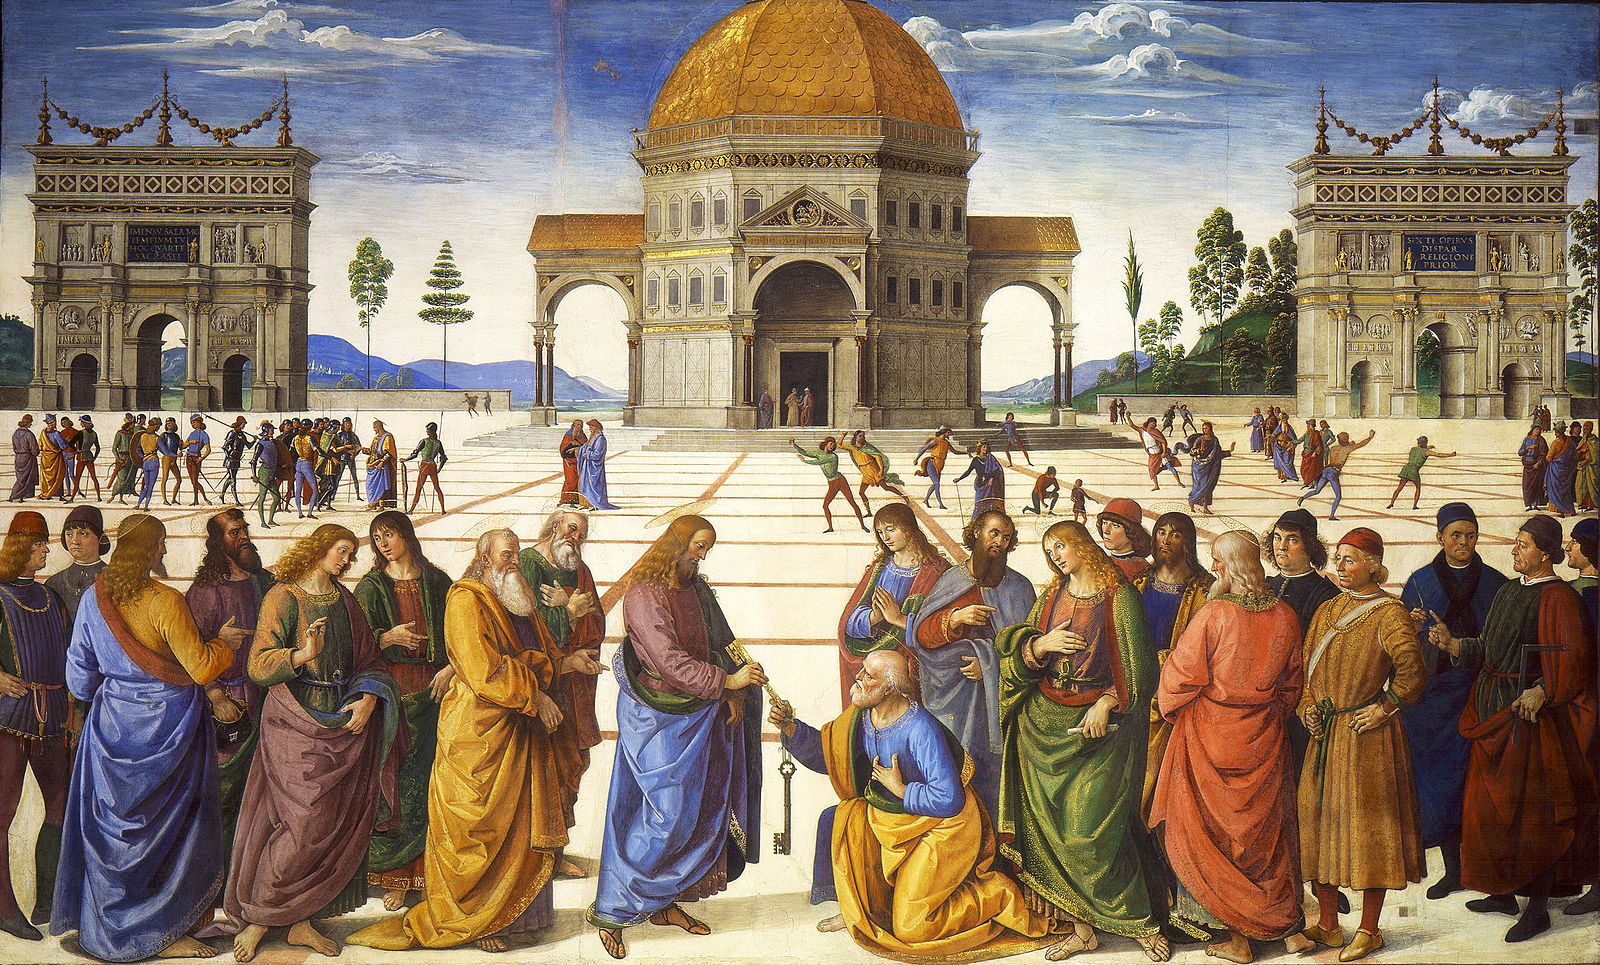
\includegraphics[width=\linewidth]{img/perugino.jpg}
  \caption{Vanishing Point Painting \cite{FileEntr24online}}\label{fig:san-pedro}
  % This work is in the public domain in its country of origin and other countries and areas where the copyright term is the author's life plus 100 years or fewer.
\endminipage\hfill
\minipage{0.5\textwidth}
  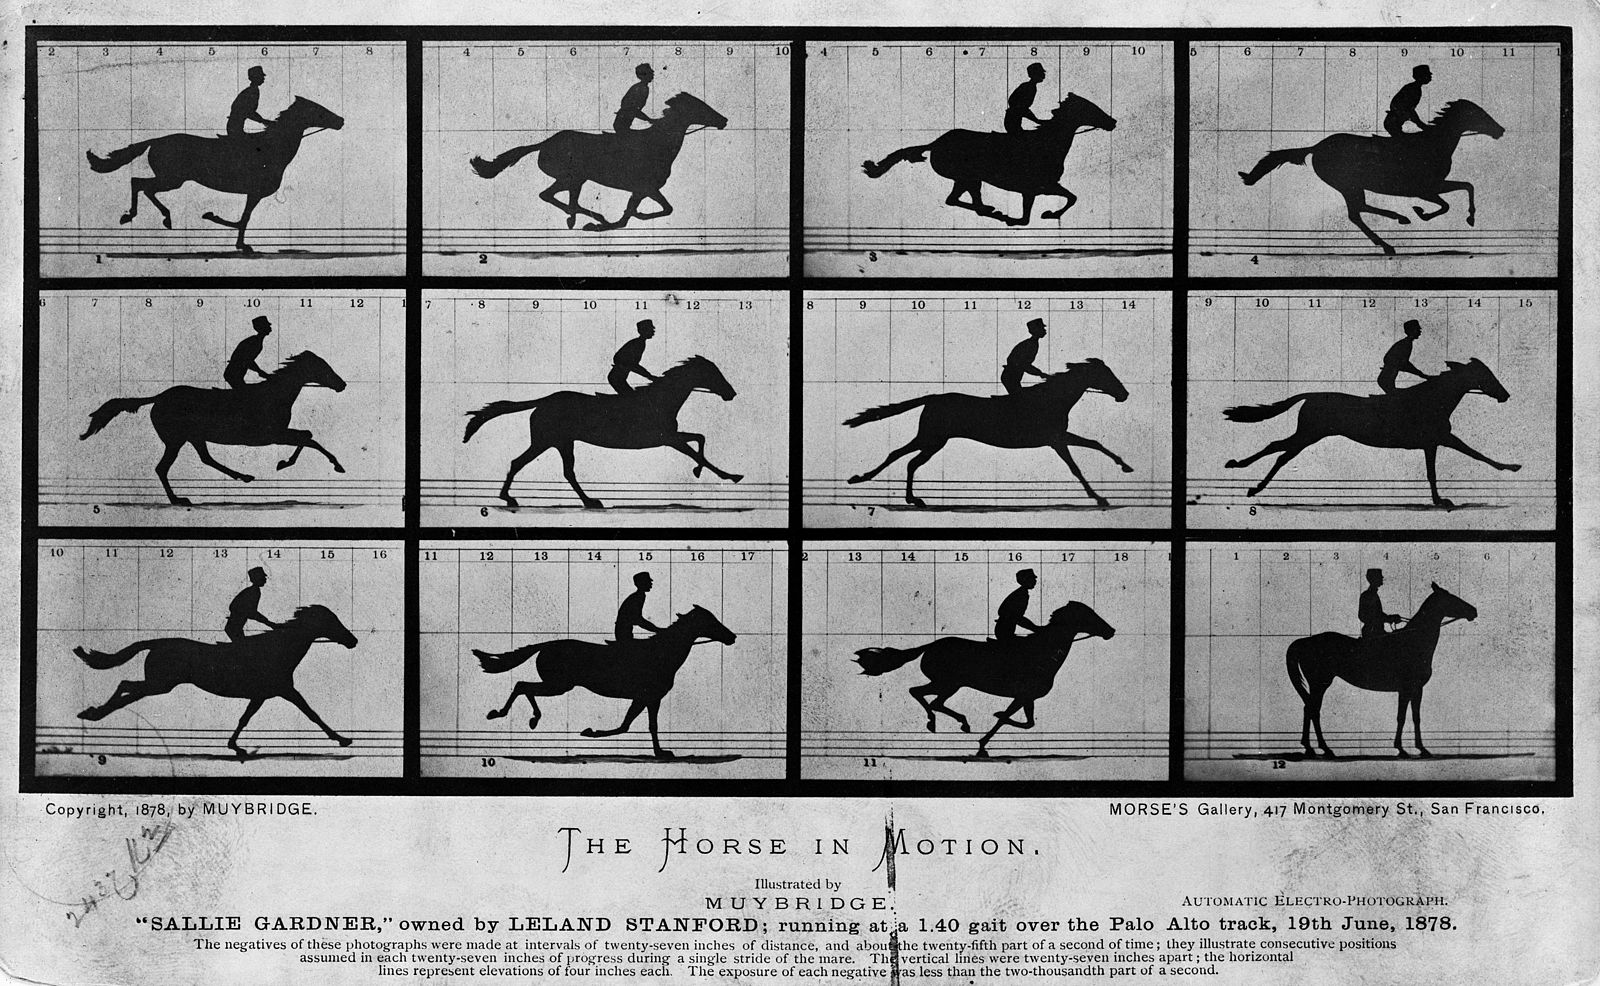
\includegraphics[width=\linewidth]{img/horse-in-mot.jpg}
  \caption{The Horse in Motion \cite{FileTheH64online}}\label{fig:horse-motion}
  % This work is in the public domain in the United States because it was published (or registered with the U.S. Copyright Office) before January 1, 1926.
\endminipage
\end{figure}

Another well known method in film-making is \textit{3D movies} which are created using special cameras and then viewed using polarized light filters creating an additional sense of depth from a 2D image. Another way to increase immersion in films is to increase the FoV of the pictures by using a wider screen. The Cinerama is an example of such a system which used three projectors to extend the FoV and projected the image upon a concave surface for a richer viewing experience. It was created in the 1950s and is a precursor to the wide, curved, UltraWide LED (Light-Emitting Diode) monitors popular today. 

These two devices however, are not as immersive as the CAVE (Cave Automatic Virtual Environment) environments developed in 1992 at the University of Illinois. In these systems a larger number of projectors are used to, ideally, cover the entire surface of the room. Some CAVE systems also use 3D video in order to improve the depth perception of the image. The benefit of this approach is that the user does not need to wear any heavy equipment on their face which might restrict their ability to move. The downside is that such environments are often very costly to set-up given the large number of projectors needed to create the visual illusion. There are similar environments which use arrays of display panels in lieu of projectors, so higher visual fidelity.

% \subsection{Head-Mounted Displays}

Much earlier, in 1965, Ivan Sutherland had introduced the concept of "The Ultimate Display", which he described as: "a room within which the computer can control the existence of matter." \cite{sutherland1965ultimate} A few years later, Sutherland and his team would build "The Sword of Damocles", regarded today as the first VR Head-Mounted Display (HMD). The display was a ceiling-suspended device capable of displaying simple "wire-frame" shapes according to the users' head movements \cite{hemstrom2020comparison}. This demonstrated for the first time in a virtual system the idea of \textit{perception of stationary}, which consists of making an object appear to be still while you move your head; in a VR system this involves updating the image to compensate for the motion.

Later, in the 1990s a number of advancements were made in the field, mainly by government agencies:

\begin{enumerate}
    \item In 1982, an advanced flight simulator called the Visually Coupled Airborne Systems simulator (VCASS) was created by the US Air-force Medical Research Laboratory.
    \item In 1984, the Virtual Visual Environment Display (VIVED) was developed by the NASA Ames research center. 
    \item In the late 1980s, the term "Virtual Reality" was coined by Jaron Lanier, founder of the Visual Programming Lab (VPL). VPL would go on to develop the DataGlove and the EyePhone HMD. "Although all normal vision is lost wearing a HMD, the data glove allows the user to hold up their gloved hand in front of their face and see a digital representation through a HMD." \cite{dixon2006history}
\end{enumerate}

\begin{figure}[ht!]%force figure here, top, strict
\centering
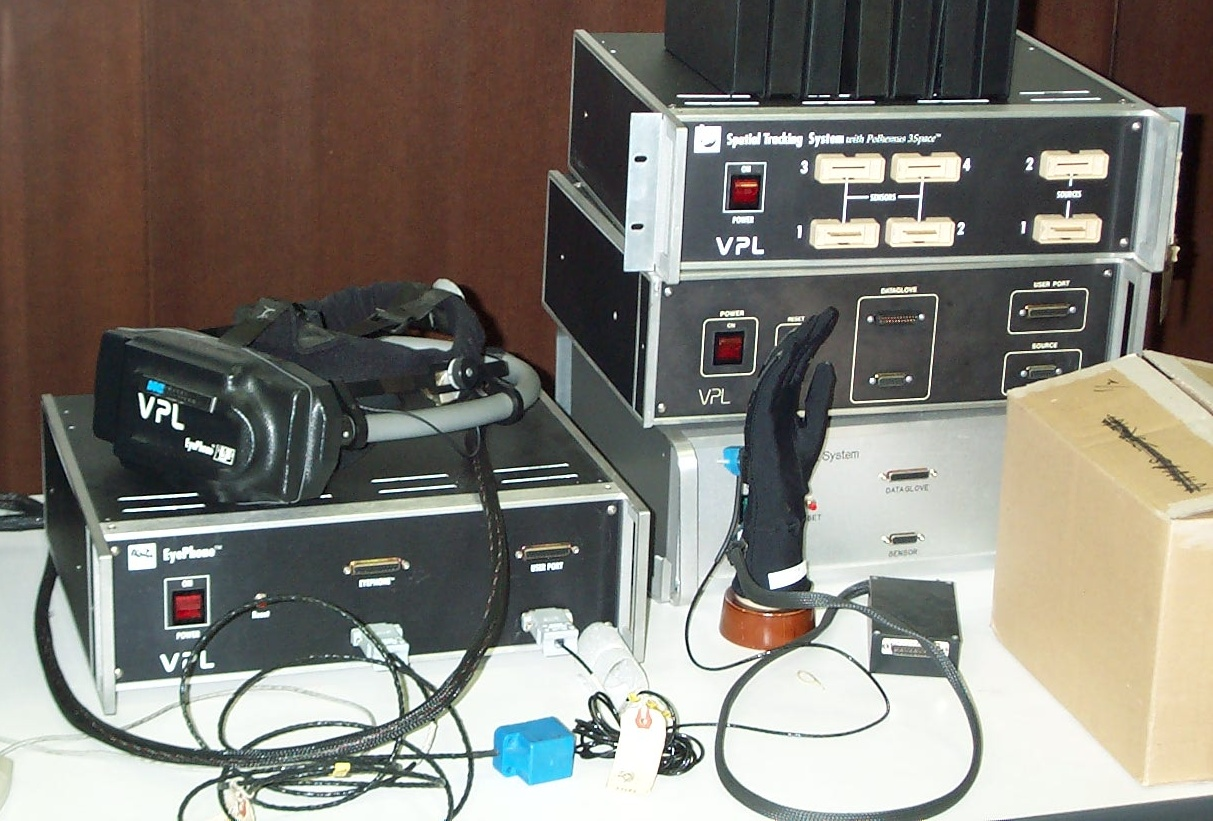
\includegraphics[width=0.7\textwidth]{img/eyephone-dataglove.jpg} 
%This work has been released into the public domain by its author, Davepape. This applies worldwide.
\caption{EyePhone HMD and DataGlove by VPL \cite{FileVPLE81online}}
\label{fig:eyephone}
\end{figure}    

Lanier went on to expand the DataGlove into a full body DataSuit, capable of tracking users' different body joints. Using these suits, multiple users were able to interact inside a a virtual environment, and even change their physical appearance. In gaming, one's virtual representation is often called his or her \textit{avatar}.

In the early 1990s, there are a small yet important number of artists who experimented with VR. Kazuhiko Hachiya created a two-person VR experience called \textit{Inter Discommunication Machine} in 1993, which switched one player's sight and sound for the others. THe idea was to confuse the borders between "you" and "me" \cite{dixon2006history}. At the Banff Centre, in Alberta, Canada, a number of VR projects were developed by a range of artists, all documented in Moser and McLeod's 1996 book "Immersed in Technology". Dixon \cite{dixon2006history} describes some of these projects in more detail.

\section{Contemporary XR Techniques}

\subsection{Hardware}

Chapter 2 of LaValle's book \cite{lavalle2016virtual} provides us with an overview of hardware practices important to VR. An important distinction LaValle makes in regards to hardware, is control in either three degrees of freedom (3DoF) or six degrees of freedom (6DoF). An ordinary object moving in 3D space has 6DoF. Three degrees of freedom correspond to its changing position in space: 

\begin{enumerate}
    \item Horizontal motion, or side-to-side motion.
    \item Vertical motion, or up-down motion.
    \item Distal motion, or close-far motion (also behind).
\end{enumerate}

The other three degrees of motion include: yaw, pitch and roll, which correspond to rotations along these three sames axes. Often the \textit{user} will be given only 3DoF in which case this is normally in the form of rotational control. This is generally the case when viewing 360 degree videos, for example. 

It is also useful to classify \textit{tracking} devices into those that offer 3DoF and 6DoF. This includes not only body tracking systems but also hand-held controllers which track user input. Some controllers, such as the Sony Playstation DualSense controller has only 3DoF, which means it sends rotational information but is not designed for positional tracking. Sony's VR ecosystem uses the Move Controller, which has an LED that is tracked by a camera system, allowing 6DoF.

\begin{figure}[!htb]
\minipage{0.5\textwidth}
  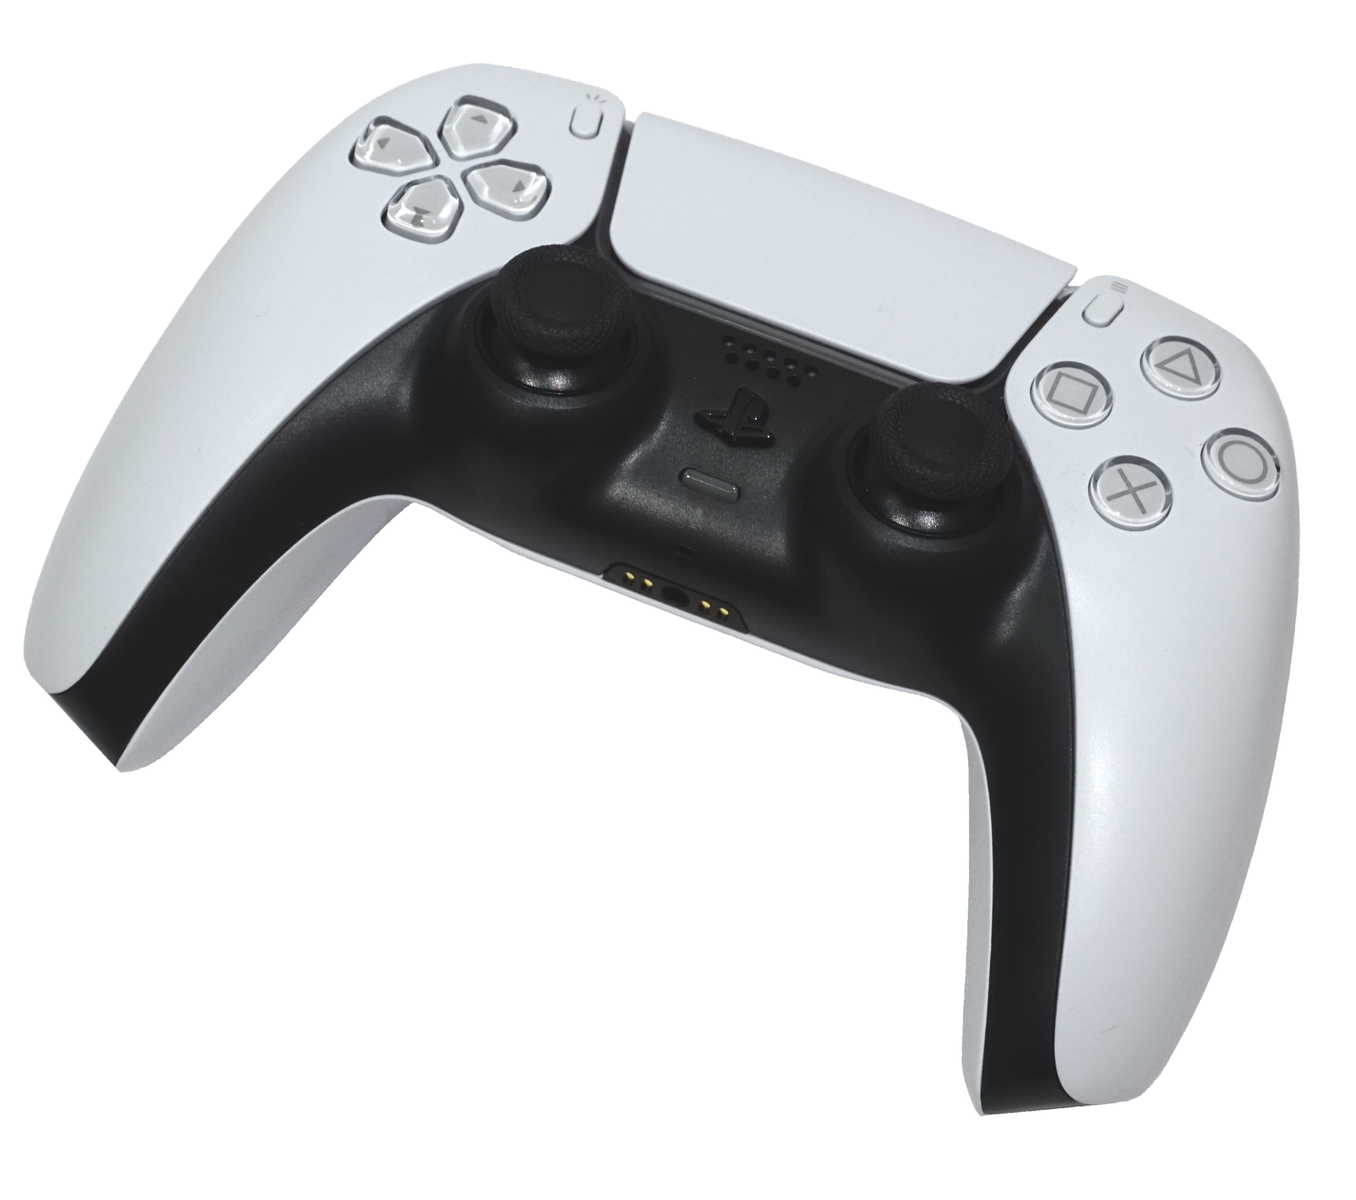
\includegraphics[width=\linewidth]{img/sony-dual.png}
  \caption{Sony DualSense Controller \cite{FilePlay5online}}\label{fig:sony-dual}
  % This file is licensed under the Creative Commons Attribution-Share Alike 4.0 International license.
\endminipage\hfill
\minipage{0.5\textwidth}
  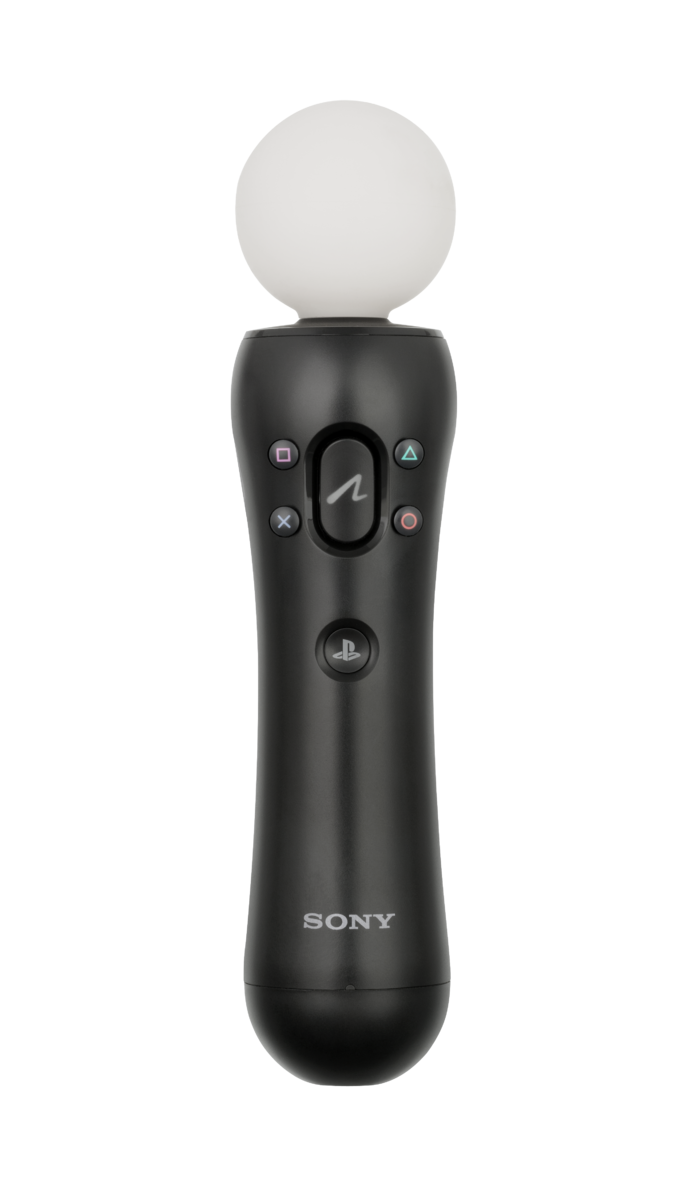
\includegraphics[width=\linewidth]{img/sony-move.png}
  \caption{Sony Move Controller \cite{FileSony89online}}\label{fig:sony-move}
  % public domain
\endminipage
\end{figure}
 
Another important distinction LaValle makes is between \textit{world-fixed} and \textit{user-fixed} systems. As we will see, user-fixed aural and visual displays offer a far more cost-effective and portable way of reproducing spatial audio and virtual scenes. World-fixed system refer to surround sound systems and CAVE-like environments, whereas user-fixed systems are personal, and refer to binocular HMD and headphone systems. Both of these approaches can be mixed and they both have their benefits and drawbacks. For sound systems some of the key trade-offs between user and world fixed systems are:

\begin{enumerate}
    \item World-fixed systems require much more power (energy). Consider the power savings from binaural reproduction versus surround sound systems. 
    \item Binaural system allow a sense of privacy, whereas surround-sound systems might disturb other people in your environment or neighbors. 
    \item User-fixed systems can be more uncomfortable if used for long periods of time, since the user is required to wear sometimes heavy electronics on their person. 
    \item World-fixed systems might allow multi-user experiences, however, there might be a noticeable drop-off in quality if users are outside the sweet-spot. Multi-user experiences are also possible over headphones, but require different sound processing for each user, which might prove computationally expensive.
    \item Headphones are often much cheaper than surround sound systems.
\end{enumerate}

The trade-offs are quite similar in the visual domain. In world-fixed environments, it will only be necessary to modify the sound and visual scene according to users directional movements. Since they are already surrounded by audio-visual stimuli, natural rotation movements should not change anything in the environment. In contrast, user-fixed environments will need to adapt to user head rotations in order to create the illusion that they are inside an encompassing environment. 

An important problem to note here is poor updating of images in VR within user-fixed experiences. The slow frame-rate, or update speed, of these systems, can cause what is known as \textit{VR sickness}. This is caused by a mismatch in sensory information coming into the brain. Over the year GPUs have become increasingly powerful, and as a result, it is possible to now update images on HMD quickly enough that VR sickness is reduced to tolerable levels. CAVE-like environments do not suffer from this problem, however, much like in surround-sound systems, there is an optimal viewing area beyond which the image will not be of good enough quality.

As \cite{lavalle2016virtual} further explains, XR systems can be divided into three primary components:

\begin{enumerate}
    \item \textbf{Displays (output):} devices that stimulate your senses. %ch 4 and 5
    \item \textbf{Sensors (input):} devices that receive and interpret information from the real world. %ch 9
    \item \textbf{Computers:} devices which process inputs and outputs.
\end{enumerate}

Given this functional delimitation we will also adopt this structure for our section on XR hardware. 

\subsubsection{Displays}

\paragraph{}

\subsubsection{Sensors}
\subsubsection{Computers}

% \subsubsection{HMDs}
% Head mounted displays.
% %https://scholar.google.com/scholar?hl=en&as_sdt=0%2C5&q=head-mounted+display+ieee&btnG=

% \subsubsection{MOCAP}
% MOtion CAPture systems. 
% %https://arxiv.org/pdf/1607.02046.pdf

% \subsubsection{360\textdegree cameras}
% % https://ieeexplore.ieee.org/stamp/stamp.jsp?arnumber=7892229&casa_token=GSr2i72N1-cAAAAA:RmRLZa4onN2qE6AMEd_Hg_0m_JcehUXB1J28wL6PzpUA89UV3ZoNXvsUqlWV5ZNHG8tF-j8Lcuzn&tag=1

% \subsubsection{CAVEs}
% %https://www.sciencedirect.com/science/article/pii/S0167739X08001167?casa_token=pOdchEnz0b0AAAAA:_5pB4ufLKxGIrH6Si-_Z3cy31P9H2ZkxIUAHbYxPW26c4rvBZhCQVLYyDcUiBFL9Ug5TZHll5-Fc

\section{Software}

%Synthetic virtual world versus real virtual world. 
%Simulataneous Localization and Mapping (SLAM)

%matched zone = safe zone
%locomotion

\subsection{Game Engines}
Unity, Unreal, Godot, etc.

\subsection{WebXR}

WebXR refers to VR or AR applications that "run" on the web. In contrast to mobile or computer applications that load assets and code from a hard disk, after the application has been downloaded, these applications dynamically, and temporarily, access data from one or more servers. The clear limitation of these systems, as a result, is that a constant, good quality, network connection is required for the experience to perform smoothly. 

WebXR has some clear benefits when compared to native XR applications that run on mobile devices or personal computers. One of the main benefits of these systems is their flexibility and interoperability across devices. What we mean by this is that, in contrast to other systems, webXR applications tend to work on just about any device that is connected to the internet, so long as a modern browser is used. 

In contrast, when one develops and builds an application for one particular operating system (OS), it is not always the case that the same application can be built seamlessly for another OS. Microsoft and Apple are the two leading companies in terms of commercial operating systems for computer devices. Most of the time, XR project developed for one operating system are not suitable for the other. This limits the artists to a segment of the population he or she would most likely wish to engage with. 

Another virtue of webXR is that a HMD is not required to attain a partial degree of immersion. There are various XR experiences built on the web for sophisticated HMDs, which can be experienced over a computer or cellphone. While not fully immersive, this allows people who feel uncomfortable with wearing HMDs to experience an artist's work, at least to a limited degree. 

\subsubsection{WebXR Audio}

Ambisonics has clear bandwidth efficiencies over pure object based solutions due to the fact the $N$ sources can be encoded into a lower number of channels, dubbed ambisonic harmonics, and then decoded binaurally. This sound field synthesis technique varies in quality depending on the order of the ambisonic system. A FOA system might reduce the amount of data required to represent a sound field, but a HOA might provide a more realistic experience given the improved spatial resolution of the system.

There is a key trade-off here that must be reconciled in order to determine what is the minimum number of ambisonic channels that are required for a suitable XR experience. In addition to this criterion, we must also consider that a number of high-quality data compression ambisonic systems are able to further reduce this data load at the expense of quality of experience (QoE). 

The data compression algorithms use perceptual features of the auditory system to reduce the amount of data required for satisfying playback. Among these algorithms, the MP3 system is perhaps the most familiar to consumers. MP3 is not well suited for spatial audio, however other compression systems exist for this task. These compression systems exploit our ear's inability to hear tones below a certain \textit{masking threshold}. When we hear a tone a narrow region of our \textit{basilar membrane} gets activated. It has been shown that when two tones, both inside this region, are played together, if one is not sufficiently loud, it will not be perceived at all. This is only one of various mechanisms artfully exploited by compression systems. Herre \cite{herre2015mpeg} provides a good overview of multi-channel data compression systems which informed the design of MPEG-H. 

Three minutes of uncompressed audio at 44,100 samples per second and 24 bits per sample results in roughly 2.2GB of audio data at 9OA. In contrast a 3OA system would result in 6 times less amount of space required, with only 0.35GB of data required to reproduce the sound field. A FOA file, with 3 minutes of music, would require roughly 0.09GB of data, or roughly 90MB. The size of the music file is an important bottleneck in fixed-media works. In cases where sound is transmitted live in an ambisonic format it is also important to determine the \textit{bitrate} of the audio stream. This is the amount of data per unit time (generally seconds) that is required for proper reproduction. 

In order to perform the binaural synthesis required for immersive VAE recreation, webXR frameworks must perform multiple convolutions with HRIRs. Convolution, even in the frequency domain, is a CPU intensive operation. In a "virtual speaker" approach to binaural decoding, two convolutions are needed for each virtual speaker. The number of virtual speakers will affect the QoE, thus a balance needs to once more been struck, this time between high "virtual speaker" count and low-CPU requirements. 

\paragraph{Resonance}

There are several implementations of binaural spatial audio online. Among them, the most popular open-source solution is Resonance. In \cite{gorzel2019efficient}, Gorzel describes some techniques to optimize HOA playback. Firstly, the author describes the implementation of a Look Up Table (LUT) instead of using $cos$ or $sin$ functions inside ones code. This way the spherical harmonic coefficients are pre-computed and can be retrieved based on the current angles of the sound source. In order to provide smooth transitions between coefficients well known interpolation schemes can be used. More importantly, however, this paper points out the possibility of exploiting spherical harmonic symmetries in order to reduce the memory requirements of the system. Gorzel points out that spherical harmonics have well-known symmetries making it possible to derive all coefficient from a single quadrant determined by the azimuth and elevation angle of the sound source. By simply calculating the front-left-top quadrant of the sphere, all the other values can be known by simply applying sign changes. 

\paragraph{JSAmbisonics}

\paragraph{Web Audio API}

% https://immersive-web.github.io/webxr-samples/explainer.html

%https://www.khronos.org/gltf/

% Most usage of WebGL today happens via frameworks that significantly simplify the creation of 3D scenes compared to using raw WebGL. Some of the more popular examples are three.js, babylon.js, and PlayCanvas. There's also frameworks that are specifically designed to create XR content on the web, such as A-Frame and ReactVR. These are all fantastic libraries with their own strengths and focuses, and in general it's recommended that you find tools that suit your needs and rely on them rather than trying to build your own rendering systems from scratch.

% However, most frameworks will also hide away the details of interacting with the WebXR API. That's generally great for users, but not terribly useful when the entire point of your code is to demonstrate how to use the API! At the same time, we don't want the WebXR logic to be obscured by hundreds of lines of WebGL calls. As a result, these samples make use of their own minimalistic rendering library that is specifically designed to highlight use of the WebXR API and de-emphasize the WebGL rendering logic. It is not recommended that you use this library in your own projects, as you will almost certainly be better served by one of the more popular, better established frameworks.



\subsection{Mobile XR}
\section{Open XR Tools }

\section{The Philosophy of "Public Domain"}
% Given our focus on the use of FOSS. 

Technology has been an important part of art-making for many decades now. With the decreasing cost of computers, and their improved potential, more people today are capable of making art with computers than ever before. The technology industry remains focused on: improving, updating, and refining its products; in order to generate profit. Unfortunately, these systems are often designed with the latest hardware and operating systems in mind, which places an economic burden on composers and musicians. Furthermore, many popular exhibits and artistic works today feature technology as a core feature of the material, which excludes those who lack access or the skills to create such content.

Software, like digital art, poses a complex economic problem. Unlike physical objects, or direct services, software and digital art can easily be duplicated at little to no cost. Intellectual Property (IP) lies at the heart of this problem as was addressed by Puckette in \cite{puckette2004owns}. In his paper, Puckette used Pure Data (Pd) as a case study of what happens when a research institution commercializes its research. In the article, Puckette argues that IRCAM's\footnote{Institut de Recherche et Coordination Acoustique/Musique.} decision to enforce its IP claims to Pd and sell it as MAX/MSP resulted in a noted drop in the credibility of the institution as a research facility. The name Pd also means Public Domain. Drawing these IP lines is anything but simple since most valuable research draws from other authors' work. Similarly, most worthwhile artworks draw inspiration from its predecessors or contemporaries.

Much like software, digital art can be difficult to price. A physical painting can be analyzed to its authenticity and a price can be set based on what the market is willing to pay for it. A digital sound file, on the other hand, can be duplicated nearly for free, and mass distribution is just as cheap. A musical score operates on basically the same principle. \cite{puckette2001new} explored the idea of bringing some seminal computer music works into the public domain by using Pd, however, not all the works are included on his website, because IRCAM insisted some of patches be taken down. This creates an interesting dilemma for the composers, who naturally would prefer their music be performed as often as possible. 

When working in the scientific domain, one of the applied principles for validating experiments is the reproduction of the research. One of the benefits of using public domain tools, like Pd, is the ability to exercise a similar principle in the artistic domain. The idea being that aesthetic musical principles are hard to extend if the technology inherent to them is proprietary. In the pedagogical domain, this idea is also extremely powerful. Using public domain tools enables one to share their teachings with a wider subset of the population, without having to consider the economic barriers that software can sometimes create. 

Fernando Lopez-Lezcano, a composer and computer scientist at Stanford, has also been interested in this dichotomy for a long time. Fernando has been building Linux distributions for sound research at CCRMA for many years now. In \cite{CEC-eCon28-online} Fernando talks about the traditions established at Stanford related to open source software and how these have evolved over the years. 

%https://econtact.ca/11_3/index.html
%https://econtact.ca/11_3/lopez_lezcano_ccrma.html

\section{The Future of XR}
\section{Conclusion}



